\chapter{Fundamentos teóricos y tecnológicos}
\label{chap:fundamentos-teoricos-tecnologicos}

Este capítulo presenta los conceptos teóricos y tecnológicos necesarios para contextualizar el desarrollo del proyecto. En primer lugar, se introduce la representación digital de juegos de tablero, prestando atención a cómo una partida física puede modelarse mediante estados, acciones y transiciones. A continuación, se revisan los fundamentos de la inteligencia artificial aplicada a juegos de dos jugadores, incluyendo los algoritmos de búsqueda adversarial más relevantes. Finalmente, se describen los conceptos principales de visión por computador necesarios para comprender la digitalización de un tablero físico mediante imágenes.

%==============================================================================
% 2.1. Juegos de tablero y representación digital
% =============================================================================
\section{Juegos de tablero y representación digital}
\label{sec:juegos-tablero-representacion-digital}

Los juegos de tablero constituyen un tipo concreto de juego de mesa en el que la partida se desarrolla sobre un espacio físico organizado, normalmente representado por un tablero dividido en posiciones, casillas o regiones. En torno a este espacio, los jugadores interactúan con piezas, fichas, cartas u otros componentes materiales siguiendo un conjunto de reglas que determina qué acciones son válidas, cómo se modifica la configuración de la partida y en qué condiciones esta llega a su fin.

Para que un juego de tablero pueda ser tratado por un sistema informático, es necesario abstraer sus elementos físicos en una representación digital. Esta representación no busca reproducir todos los detalles materiales del juego, como la apariencia exacta del tablero o la forma de sus componentes, sino conservar la información necesaria para aplicar sus reglas. De este modo, el tablero físico se convierte en una estructura formal sobre la que el programa puede comprobar movimientos, actualizar la partida y mantener una descripción coherente de su evolución.

Desde el punto de vista computacional, un juego puede definirse formalmente como un problema de búsqueda. Russell y Norvig describen esta formulación mediante una serie de componentes básicos~\cite{russell2020aima}:

\begin{itemize}
    \item \textbf{Estado inicial}: describe la configuración de partida e identifica el jugador al que corresponde mover.
    \item \textbf{Función sucesora}: devuelve, para un estado dado, las parejas formadas por un movimiento legal y el estado resultante tras aplicarlo.
    \item \textbf{Prueba terminal}: determina si la partida ha finalizado. Los estados en los que el juego ha terminado se denominan estados terminales.
    \item \textbf{Función de utilidad}: asigna un valor a los estados terminales, representando el resultado de la partida desde el punto de vista considerado.
\end{itemize}

A partir de esta formulación, una partida puede entenderse como una secuencia de estados conectados por acciones legales. Cada acción aplicada sobre un estado produce un nuevo estado, dando lugar a una transición. La partida avanza mediante estas transiciones hasta alcanzar, en su caso, un estado terminal asociado a un resultado.

El estado de juego representa una descripción lógica de una posición concreta de la partida. En un juego de tablero, este estado suele incluir la ubicación de las piezas, el turno actual, los recursos disponibles para cada jugador y cualquier otra información necesaria para aplicar correctamente las reglas.

A partir del estado actual, las reglas del juego determinan el conjunto de acciones legales. Esta distinción es fundamental, ya que no toda modificación posible del tablero constituye un movimiento válido. Aunque en un entorno físico un jugador pueda desplazar una pieza manualmente a una posición cualquiera, el modelo digital debe ser capaz de comprobar si esa acción respeta las restricciones del juego. En este sentido, la representación digital convierte las reglas en condiciones verificables por el sistema.

En los juegos por turnos, esta forma de modelar la evolución de la partida resulta especialmente natural. Cada jugador actúa en un momento determinado y cada movimiento modifica la posición sobre la que se tomará la siguiente decisión.

Además de representar posiciones intermedias, el modelo digital debe identificar cuándo la partida ha terminado. Para ello se reconocen estados terminales, es decir, situaciones en las que ya no es necesario continuar aplicando acciones. Estos estados suelen estar asociados a un resultado, como la victoria de un jugador, la derrota del otro o, en determinados juegos, un empate. La detección de estas condiciones permite validar el desarrollo de la partida y comunicar su desenlace al resto del sistema.

En conjunto, la representación digital proporciona una base formal sobre la que el sistema puede aplicar las reglas del juego y coordinar los módulos posteriores. Al separar la información relevante de los elementos físicos, el tablero deja de tratarse como un objeto material y pasa a describirse como una estructura lógica sobre la que pueden operar técnicas de inteligencia artificial y visión por computador.


%==============================================================================
% 2.2. Inteligencia artificial en juegos de dos jugadores
% =============================================================================
\section{Inteligencia artificial en juegos de dos jugadores}
\label{sec:inteligencia-artificial-juegos-dos-jugadores}

Una vez que un juego ha sido representado digitalmente mediante estados, acciones legales y transiciones, es posible aplicar técnicas de inteligencia artificial para seleccionar acciones de forma automática. En este contexto, el objetivo no consiste únicamente en ejecutar movimientos válidos, sino en escoger aquellos que resulten más favorables de acuerdo con el estado actual de la partida y sus posibles consecuencias futuras.

\subsection{Juegos como entornos adversariales}

Un juego de dos jugadores puede entenderse como un entorno de decisión en el que varios agentes actúan sobre un mismo estado compartido. Cada jugador elige sus acciones de acuerdo con sus propios objetivos, y dichas acciones modifican la situación sobre la que deberá decidir el rival en su turno. Por ello, el efecto de una jugada no puede analizarse de forma aislada, ya que también depende de las respuestas que puede provocar en el oponente.

En los juegos competitivos, esta interacción adquiere carácter adversarial, puesto que el avance de un jugador suele producirse en oposición al del otro. Una acción aparentemente favorable puede dejar una posición vulnerable si facilita una respuesta ventajosa del rival. En consecuencia, la decisión automática no debe limitarse a comprobar qué movimientos son legalmente posibles, sino que debe considerar la presencia de un oponente que también intenta mejorar su propia situación.

Esta perspectiva permite formular la partida como una secuencia de decisiones alternas entre dos participantes con intereses enfrentados. A partir de esta idea, resulta necesario estudiar qué propiedades del juego permiten modelar formalmente el problema y aplicar métodos de razonamiento adecuados para la toma de decisiones.


\subsection{Propiedades del modelo de juego}

Muchos juegos de tablero competitivos pueden estudiarse dentro de una categoría especialmente adecuada para la inteligencia artificial clásica: los juegos deterministas, por turnos, de información perfecta y, en muchos casos, de suma cero. Este marco permite describir la toma de decisiones de manera precisa y facilita el análisis de la partida desde un punto de vista computacional.

\begin{itemize}
    \item \textbf{Determinismo}: un juego es determinista cuando el resultado de una acción queda completamente determinado por el estado actual y por las reglas del juego. En este tipo de juegos no intervienen elementos aleatorios que alteren el resultado de una jugada, como dados, cartas ocultas robadas al azar o eventos externos. Por tanto, si se conoce el estado actual y la acción realizada, el estado resultante puede calcularse de forma precisa.

    \item \textbf{Turnos}: un juego por turnos es aquel en el que los jugadores actúan de forma alterna o secuencial. Cada jugador realiza una acción en su turno y modifica el estado sobre el que actuará el siguiente participante. Esta estructura se adapta de forma natural al razonamiento computacional, ya que la partida puede analizarse como una sucesión ordenada de decisiones.

    \item \textbf{Información perfecta}: en un juego de información perfecta, los jugadores conocen el estado completo de la partida en el momento de tomar una decisión. En este tipo de juegos, los agentes actúan secuencialmente y observan el estado del mundo antes de decidir qué acción realizar~\cite{poole2023foundations}. Esta propiedad los diferencia de juegos con información oculta o privada, donde un jugador puede desconocer parte de la situación real.

    \item \textbf{Suma cero}: en los juegos de suma cero, los intereses de los jugadores están directamente enfrentados. Una mejora en el resultado de un jugador implica un empeoramiento equivalente en el resultado del otro. En juegos de dos agentes de suma cero, una recompensa positiva para un agente se corresponde con una recompensa negativa para el otro~\cite{poole2023foundations}. Esta propiedad permite interpretar la partida como un conflicto directo entre objetivos opuestos.
\end{itemize}

Estas propiedades son especialmente relevantes en nuestro proyecto, ya que la partida puede describirse como una sucesión de turnos sin azar y con información visible para ambos jugadores. Esto permite que el sistema trate cada posición como un estado bien definido sobre el que aplicar reglas y seleccionar acciones legales.


%==============================================================================
% 2.3. Algoritmos de búsqueda adversarial
% =============================================================================
\section{Algoritmos de búsqueda adversarial}
\label{sec:algoritmos-busqueda-adversarial}

\subsection{Árbol de juego}

El árbol de juego es una representación de las posibles continuaciones de una partida a partir de un estado determinado. La raíz del árbol corresponde al estado actual, cada rama representa una acción legal y cada nodo hijo representa el estado resultante tras aplicar dicha acción. Al expandir sucesivamente los estados alcanzables, el árbol describe las diferentes secuencias de movimientos que podrían producirse durante la partida.

En un juego por turnos de dos jugadores, los niveles del árbol suelen alternar entre ambos participantes. Un nivel representa las decisiones disponibles para el jugador que debe mover en ese momento, mientras que el siguiente nivel representa las posibles respuestas del oponente. De este modo, el árbol no solo muestra las acciones inmediatas, sino también las consecuencias que pueden derivarse de ellas tras varios turnos.

Las hojas del árbol pueden corresponder a estados terminales, cuando la partida ha finalizado, o a estados intermedios cuando la búsqueda se detiene antes de llegar al final. En el primer caso, el valor del estado puede obtenerse directamente a partir del resultado de la partida. En el segundo caso, es necesario estimar la calidad de la posición mediante una función de evaluación, aspecto que se tratará más adelante.

Aunque el árbol de juego proporciona una representación clara del problema, su tamaño puede crecer rápidamente. Si en cada estado existen varias acciones legales, el número de nodos aumenta de forma exponencial con la profundidad de búsqueda. Esta expansión combinatoria hace que, en muchos juegos, no sea viable explorar todas las partidas posibles hasta llegar a estados terminales. Por este motivo, los algoritmos de búsqueda adversarial incorporan técnicas para seleccionar, limitar u optimizar la exploración del árbol~\cite{russell2020aima,poole2023foundations}.


\subsection{Algoritmo minimax}

El algoritmo minimax es uno de los métodos clásicos para la toma de decisiones en juegos de dos jugadores, deterministas, por turnos y de suma cero. El concepto minimax tiene su origen en la teoría de juegos, especialmente en los trabajos de John von Neumann sobre juegos de dos personas con intereses opuestos~\cite{kjeldsen2001minimax}. En inteligencia artificial, se utiliza habitualmente como un procedimiento de búsqueda sobre árboles de juego para seleccionar movimientos bajo la hipótesis de que ambos jugadores actúan de forma racional~\cite{russell2020aima,poole2023foundations}. En este contexto, un jugador intenta maximizar el valor de la posición, mientras que el adversario intenta minimizarlo.

El funcionamiento general del algoritmo puede resumirse en los siguientes pasos:

\begin{enumerate}
    \item Se construye, de forma explícita o implícita, el árbol de juego a partir del estado actual.
    \item Se asigna un valor a los nodos hoja, ya sea porque representan estados terminales o porque se ha alcanzado una profundidad máxima de búsqueda.
    \item En los niveles correspondientes al jugador maximizador, se selecciona el mayor valor entre los nodos sucesores.
    \item En los niveles correspondientes al jugador minimizador, se selecciona el menor valor entre los nodos sucesores.
    \item Los valores se propagan desde las hojas hacia la raíz, permitiendo elegir la acción inicial con mejor valor minimax.
\end{enumerate}

La Figura~\ref{fig:minimax-tree} muestra un ejemplo sencillo de propagación de valores. Los nodos hoja contienen evaluaciones numéricas de distintas posiciones. En primer lugar, cada nodo de minimización selecciona el menor valor entre sus hijos. Después, la raíz, correspondiente al jugador maximizador, selecciona el mayor valor entre los valores propagados por sus sucesores.

\vspace{0.5cm}

\begin{figure}[htbp]
\centering
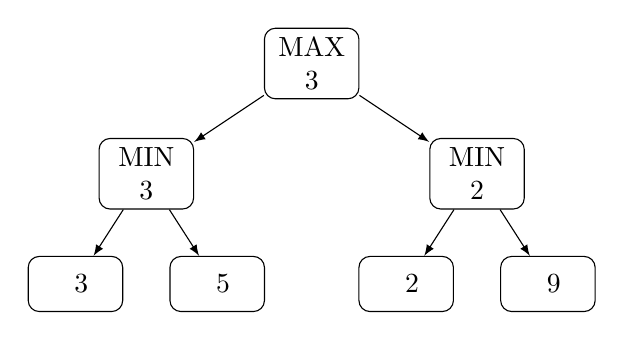
\begin{tikzpicture}[
    level distance=1.4cm,
    level 1/.style={sibling distance=4.2cm},
    level 2/.style={sibling distance=1.8cm},
    every node/.style={
        draw,
        rounded corners,
        align=center,
        minimum width=1.2cm,
        minimum height=0.7cm
    },
    edge from parent/.style={draw, -latex}
]
\node {MAX\\$3$}
    child {node {MIN\\$3$}
        child {node {\hspace{1.5mm}$3$}}
        child {node {\hspace{1.5mm}$5$}}
    }
    child {node {MIN\\$2$}
        child {node {\hspace{1.5mm}$2$}}
        child {node {\hspace{1.5mm}$9$}}
    };
\end{tikzpicture}
\caption{Ejemplo de propagación de valores en el algoritmo minimax.}
\label{fig:minimax-tree}
\end{figure}
\vspace{1cm}


El Algoritmo~\ref{alg:minimax} muestra una versión simplificada de minimax, adaptada a una búsqueda con profundidad limitada a partir de la formulación clásica del algoritmo~\cite{russell2020aima}. La función recibe un estado, una profundidad restante y un indicador que determina si el turno corresponde al jugador maximizador o al minimizador. Si el estado es terminal o se ha alcanzado la profundidad límite, se devuelve una evaluación del estado. En caso contrario, se exploran las acciones legales y se propaga el valor máximo o mínimo según el jugador que deba actuar.

\vspace{0.3cm}
\begin{algorithm}[H]
\caption{Algoritmo minimax}
\label{alg:minimax}
\begin{algorithmic}[1]
\State \textbf{Entrada:} estado de juego $s$, profundidad restante $d$, indicador $maximizando$
\State \textbf{Salida:} valor estimado del estado $s$
\If{$s$ es terminal \textbf{o} $d = 0$}
    \State \Return $evaluar(s)$
\EndIf
\If{$maximizando$}
    \State $mejor \gets -\infty$
    \ForAll{acción legal $a$ en $s$}
        \State $s' \gets resultado(s, a)$
        \State $mejor \gets \max(mejor, minimax(s', d - 1, false))$
    \EndFor
    \State \Return $mejor$
\Else
    \State $mejor \gets +\infty$
    \ForAll{acción legal $a$ en $s$}
        \State $s' \gets resultado(s, a)$
        \State $mejor \gets \min(mejor, minimax(s', d - 1, true))$
    \EndFor
    \State \Return $mejor$
\EndIf
\end{algorithmic}
\end{algorithm}

En juegos de suma cero, minimax puede expresarse también mediante la formulación \textbf{negamax}. Esta variante aprovecha que el valor de una posición para un jugador es el opuesto del valor de esa misma posición para el adversario. De este modo, en lugar de alternar explícitamente entre una función de maximización y otra de minimización, la búsqueda puede formularse como una única función que maximiza el valor negativo del estado resultante desde la perspectiva del rival. Conceptualmente, negamax no cambia el criterio de decisión de minimax, sino que ofrece una forma más compacta de expresarlo en juegos con utilidad opuesta para ambos jugadores.

La principal ventaja de minimax es que proporciona un criterio claro para decidir en juegos adversariales. Sin embargo, su coste computacional puede ser elevado, ya que el número de nodos crece rápidamente con la profundidad de búsqueda. Por ello, en la práctica suele combinarse con límites de profundidad, funciones heurísticas y técnicas de optimización.


\subsection{Poda alfa-beta}

La poda alfa-beta es una optimización del algoritmo minimax que permite reducir el número de nodos explorados en el árbol de juego sin modificar la decisión final obtenida. La idea principal consiste en dejar de analizar aquellas ramas que no pueden influir en el valor que finalmente será seleccionado por minimax. Por tanto, alfa-beta no cambia el criterio de decisión del algoritmo, sino la eficiencia con la que se recorre el árbol~\cite{russell2020aima,poole2023foundations}.

El algoritmo mantiene dos valores durante la búsqueda: $\alpha$ y $\beta$. El valor $\alpha$ representa la mejor alternativa encontrada hasta el momento para el jugador maximizador, mientras que $\beta$ representa la mejor alternativa encontrada hasta el momento para el jugador minimizador. Si durante la exploración se detecta que un nodo no puede mejorar la decisión ya disponible para alguno de los jugadores, el resto de sus sucesores puede descartarse sin necesidad de evaluarlos.

El funcionamiento de la poda alfa-beta puede resumirse en los siguientes pasos:

\begin{enumerate}
    \item Se recorre el árbol de juego de forma similar a minimax, alternando entre niveles de maximización y minimización.
    \item Durante la búsqueda, se actualiza $\alpha$ con el mejor valor encontrado hasta el momento para el jugador maximizador.
    \item Del mismo modo, se actualiza $\beta$ con el mejor valor encontrado hasta el momento para el jugador minimizador.
    \item Si en algún momento se cumple que $\alpha \geq \beta$, la rama actual deja de poder afectar al resultado final y se interrumpe su exploración.
    \item El valor devuelto por el algoritmo es el mismo que devolvería minimax, pero normalmente habiendo evaluado menos nodos.
\end{enumerate}

La Figura~\ref{fig:alphabeta-pruning} muestra un ejemplo simplificado de esta idea. Una vez que el primer subárbol ha proporcionado a la raíz una alternativa con valor $3$, el segundo nodo de minimización encuentra un sucesor con valor $2$. Dado que el jugador minimizador escogería como máximo un valor menor o igual que $2$ en ese subárbol, dicha rama ya no puede mejorar la opción disponible para el jugador maximizador. Por ello, el resto de sucesores del nodo puede descartarse sin alterar la decisión final.

\vspace{0.5cm}
\begin{figure}[H]
\centering
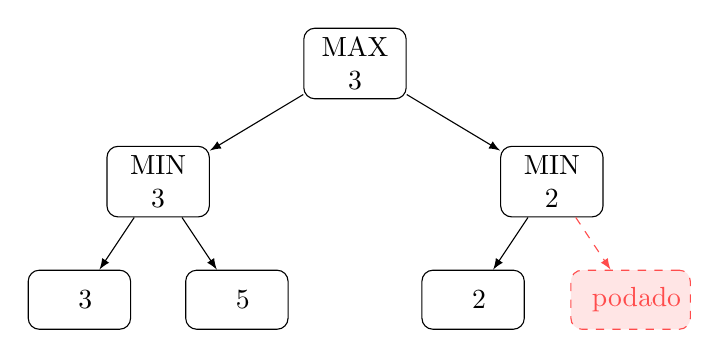
\begin{tikzpicture}[
    level distance=1.5cm,
    level 1/.style={sibling distance=5.0cm},
    level 2/.style={sibling distance=2.0cm},
    normal/.style={
        draw,
        rounded corners,
        align=center,
        minimum width=1.3cm,
        minimum height=0.75cm,
    },
    pruned/.style={
        draw=red!70,
        rounded corners,
        align=center,
        minimum width=1.3cm,
        minimum height=0.75cm,
        fill=red!10,
        text=red!70
    },
    edge from parent/.style={draw, -latex},
    prunededge/.style={draw=red!70, dashed, -latex}
]

\node[normal] {MAX\\$3$}
    child {node[normal] {MIN\\$3$}
        child {node[normal] {\hspace{1.5mm}$3$}}
        child {node[normal] {\hspace{1.5mm}$5$}}
    }
    child {node[normal] {MIN\\$2$}
        child {node[normal] {\hspace{1.5mm}$2$}}
        child[prunededge] {node[pruned] {\hspace{1.5mm}podado}}
    };

\end{tikzpicture}
\caption{Ejemplo de poda alfa-beta en un árbol minimax.}
\label{fig:alphabeta-pruning}
\end{figure}
\vspace{0.8cm}

El Algoritmo~\ref{alg:alphabeta} muestra una versión simplificada de minimax con poda alfa-beta. Al igual que en el caso anterior, se utiliza una profundidad máxima de búsqueda y una función de evaluación para los estados terminales o para aquellos estados en los que se alcanza el límite de profundidad. La diferencia principal respecto a minimax es la actualización de los valores $\alpha$ y $\beta$, que permiten detectar cuándo una rama puede ser descartada.

\begin{algorithm}[H]
\caption{Minimax con poda alfa-beta}
\label{alg:alphabeta}
\begin{algorithmic}[1]
\State \textbf{Entrada:} estado de juego $s$, profundidad restante $d$, valores \textcolor{blue}{$\alpha$ y $\beta$}, indicador $maximizando$
\State \textbf{Salida:} valor estimado del estado $s$
\If{$s$ es terminal \textbf{o} $d = 0$}
    \State \Return $evaluar(s)$
\EndIf
\If{$maximizando$}
    \State $mejor \gets -\infty$
    \ForAll{acción legal $a$ en $s$}
        \State $s' \gets resultado(s, a)$
        \State $mejor \gets \max(mejor, alphabeta(s', d - 1, \textcolor{blue}{\alpha}, \textcolor{blue}{\beta}, false))$
        \State \textcolor{blue}{$\alpha \gets \max(\alpha, mejor)$}
        \If{\textcolor{blue}{$\alpha \geq \beta$}}
            \State \textcolor{blue}{\textbf{break}}
        \EndIf
    \EndFor
    \State \Return $mejor$
\Else
    \State $mejor \gets +\infty$
    \ForAll{acción legal $a$ en $s$}
        \State $s' \gets resultado(s, a)$
        \State $mejor \gets \min(mejor, alphabeta(s', d - 1, \textcolor{blue}{\alpha}, \textcolor{blue}{\beta}, true))$
        \State \textcolor{blue}{$\beta \gets \min(\beta, mejor)$}
        \If{\textcolor{blue}{$\alpha \geq \beta$}}
            \State \textcolor{blue}{\textbf{break}}
        \EndIf
    \EndFor
    \State \Return $mejor$
\EndIf
\end{algorithmic}
\end{algorithm}

La poda alfa-beta constituye una de las optimizaciones clásicas de minimax en árboles de juego~\cite{knuth1975alphabeta}. Su utilidad práctica no depende únicamente de las condiciones de corte descritas, sino también de su integración con estrategias que mejoran el recorrido del árbol. Estas técnicas, presentadas más adelante, no modifican el criterio de decisión del algoritmo, pero pueden reducir el coste computacional de la búsqueda y permitir alcanzar mayores profundidades en motores de juego.


\subsection{Profundidad limitada y funciones heurísticas}

Aunque minimax y la poda alfa-beta proporcionan un marco claro para tomar decisiones en juegos adversariales, en muchos juegos no resulta viable explorar el árbol completo hasta alcanzar estados terminales. El número de nodos crece rápidamente con la profundidad de búsqueda, ya que cada acción legal puede dar lugar a nuevos estados y cada uno de ellos genera, a su vez, nuevas posibilidades. Por este motivo, incluso en juegos con reglas relativamente sencillas, analizar todas las partidas posibles puede ser computacionalmente inasumible.

Para abordar esta limitación, es habitual utilizar una búsqueda con profundidad limitada. En lugar de expandir el árbol hasta el final de la partida, el algoritmo se detiene tras alcanzar una profundidad máxima. En este contexto, dicha profundidad suele medirse en \emph{ply}, término que representa un movimiento individual de uno de los jugadores dentro del árbol de juego. Por tanto, una búsqueda de varios \emph{ply} permite analizar secuencias alternas de acciones propias y respuestas del adversario. Esta limitación reduce el coste computacional y permite controlar el tiempo dedicado a la toma de decisiones.

El uso de profundidad limitada plantea un nuevo problema: al detener la búsqueda antes de alcanzar estados terminales, el algoritmo ya no dispone de un resultado definitivo de victoria, derrota o empate. Por tanto, es necesario estimar la calidad de las posiciones alcanzadas en la frontera de búsqueda. Esta estimación se realiza mediante una función heurística de evaluación, que asigna un valor numérico a un estado no terminal en función de características consideradas relevantes para el juego~\cite{russell2020aima,poole2023foundations}.

Una función heurística no garantiza conocer el resultado real de la partida desde una posición concreta, sino que proporciona una aproximación útil para orientar la búsqueda. En juegos de tablero, estas funciones suelen combinar distintos criterios, entre los que pueden encontrarse:

\begin{itemize}
    \item \textbf{Ventaja material}: diferencia entre las piezas o recursos disponibles para cada jugador.
    \item \textbf{Movilidad}: número o calidad de las acciones legales disponibles.
    \item \textbf{Seguridad}: grado de protección de piezas o posiciones importantes.
    \item \textbf{Control del tablero}: influencia sobre zonas relevantes del espacio de juego.
    \item \textbf{Proximidad a la victoria}: cercanía a una condición que permita finalizar favorablemente la partida.
\end{itemize}

La elección de estos factores depende de las características del juego y condiciona en gran medida el comportamiento del agente.

Desde el punto de vista de minimax, la función heurística sustituye a la función de utilidad cuando la búsqueda no llega a un estado terminal. Los valores estimados en la frontera del árbol se propagan entonces hacia la raíz mediante el mismo procedimiento de maximización y minimización. De este modo, el algoritmo puede seleccionar una acción aunque solo haya explorado una parte limitada del espacio de juego.

La calidad de una inteligencia artificial basada en búsqueda depende, por tanto, de un equilibrio entre profundidad y evaluación. Una búsqueda más profunda permite considerar consecuencias más lejanas, pero requiere más tiempo de cómputo. Una función heurística más precisa puede compensar parcialmente una búsqueda menos profunda, aunque también puede introducir errores si valora incorrectamente una posición. Este equilibrio entre coste computacional y calidad de la evaluación es uno de los aspectos fundamentales en el diseño de agentes para juegos de tablero.


\subsection{Técnicas de optimización de la búsqueda}

Además de la poda alfa-beta, los motores basados en búsqueda suelen incorporar técnicas complementarias para mejorar la eficiencia del recorrido del árbol o la calidad de las evaluaciones realizadas en la frontera de búsqueda. Schaeffer agrupa muchas de estas mejoras en torno a tres ideas principales: ordenar mejor los movimientos, reducir el tamaño de la ventana de búsqueda y reutilizar información obtenida en búsquedas anteriores~\cite{schaeffer1989historyHeuristic}. Estas técnicas no modifican el problema de decisión adversarial, pero permiten aprovechar mejor el tiempo de cómputo disponible.

\begin{itemize}
    \item \textbf{Ordenación de movimientos}: la eficacia de alfa-beta depende en gran medida del orden en que se exploran las acciones. Si las jugadas más prometedoras se analizan primero, los cortes pueden producirse antes y se reduce el número de nodos evaluados. Por ello, muchos motores utilizan heurísticas para priorizar ciertos movimientos, como capturas, amenazas o jugadas que en búsquedas anteriores han producido buenos resultados. Schaeffer estudia precisamente la \emph{history heuristic}, una técnica que acumula información sobre movimientos que han sido útiles en otras partes del árbol y la utiliza para ordenar movimientos en nodos posteriores~\cite{schaeffer1989historyHeuristic}.

    \item \textbf{Tablas de transposición}: en un árbol de juego, una misma posición puede alcanzarse mediante distintas secuencias de movimientos. Las tablas de transposición aprovechan esta propiedad almacenando información de estados ya explorados, como el valor calculado, la profundidad de búsqueda utilizada o el mejor movimiento encontrado. Si la misma posición aparece de nuevo, el algoritmo puede reutilizar esa información para evitar búsquedas repetidas, ajustar los límites de alfa-beta o probar primero un movimiento previamente considerado prometedor~\cite{schaeffer1989historyHeuristic, marsland1986gameTreePruning}.

    \item \textbf{Profundización iterativa}: en lugar de ejecutar directamente una búsqueda a una profundidad fija, la profundización iterativa realiza búsquedas sucesivas de profundidad creciente. Por ejemplo, primero se explora a un ply, después a dos, luego a tres, y así sucesivamente hasta alcanzar el límite deseado o agotar el tiempo disponible. Aunque pueda parecer redundante, esta técnica permite disponer siempre de una mejor jugada parcial si la búsqueda debe detenerse y, además, proporciona información útil para ordenar movimientos en iteraciones posteriores~\cite{schaeffer1989historyHeuristic, marsland1986gameTreePruning}.

    \item \textbf{Ventanas de aspiración}: en una búsqueda alfa-beta habitual, los valores iniciales de $\alpha$ y $\beta$ pueden cubrir un intervalo muy amplio. Las ventanas de aspiración utilizan una ventana más estrecha alrededor de una estimación previa del valor esperado de la posición. Si el valor real cae dentro de esa ventana, la búsqueda puede completarse con menor coste; si queda fuera, es necesario repetir la búsqueda con límites más amplios. Esta técnica puede mejorar la eficiencia, aunque depende de que la estimación inicial sea suficientemente precisa~\cite{schaeffer1989historyHeuristic, marsland1986gameTreePruning}.

    \item \textbf{Búsqueda quiescente}: al utilizar profundidad limitada, el algoritmo puede detenerse en una posición tácticamente inestable, por ejemplo justo antes de una captura o de una amenaza importante. Evaluar directamente ese estado puede producir una estimación engañosa. La búsqueda quiescente intenta reducir este problema extendiendo selectivamente la búsqueda en posiciones no estables hasta alcanzar estados más tranquilos, donde la función de evaluación pueda aplicarse con mayor fiabilidad. Marsland relaciona esta técnica con la reducción del efecto horizonte, que aparece cuando una pérdida inevitable queda artificialmente desplazada más allá de la profundidad máxima de búsqueda~\cite{marsland1986gameTreePruning}.
\end{itemize}

En conjunto, los algoritmos y técnicas descritos en esta sección proporcionan la base del agente de inteligencia artificial desarrollado en este proyecto. Al modelar Onitama como un juego adversarial de turnos alternos, cada posición puede analizarse mediante un árbol de posibles continuaciones. Sin embargo, para que esta búsqueda sea viable en la práctica, es necesario combinar el criterio de decisión de minimax con una profundidad limitada, una función heurística de evaluación, poda alfa-beta y técnicas de optimización del recorrido. De este modo, el sistema puede seleccionar acciones legales de forma automática, equilibrando la calidad de la decisión con el tiempo de cálculo disponible.


%==============================================================================
% 2.4. Captura y normalización de la escena física.
% =============================================================================
\section{Captura y normalización de la escena física}
\label{sec:captura-normalizacion-escena-fisica}


\subsection{Captura visual del tablero}

La aplicación de visión por computador a un tablero físico parte de una diferencia fundamental entre la escena real y la información disponible para el sistema: la cámara no recibe directamente objetos, casillas o posiciones, sino una imagen bidimensional. Esta imagen es el resultado de un proceso de formación en el que intervienen la geometría de la escena, la iluminación, las propiedades de las superficies, la óptica de la cámara y la discretización realizada por el sensor~\cite{szeliski2022computerVision}. Por ello, el análisis visual del tablero debe partir de una observación condicionada por el modo en que la escena física se proyecta y se registra como imagen.

En un entorno físico, la observación del tablero no suele ser completamente limpia ni constante. Pequeños cambios en la posición de la cámara, variaciones de luz, sombras, reflejos sobre las cartas o movimientos de la mano del jugador pueden modificar de forma significativa la imagen capturada, aunque la situación lógica del juego no haya cambiado. Esta diferencia entre la estabilidad del juego y la variabilidad de la imagen es uno de los principales retos al utilizar una cámara como mecanismo de entrada.

Los juegos de tablero presentan, no obstante, una ventaja importante desde el punto de vista visual: la escena suele organizarse alrededor de una superficie plana y de regiones espaciales bien definidas. La existencia de un tablero permite buscar una referencia geométrica estable sobre la que interpretar el resto de elementos. En lugar de analizar la imagen como una escena completamente libre, puede aprovecharse la estructura del tablero para restringir el problema a una zona concreta y relacionar los elementos observados con regiones conocidas de la superficie de juego.

Existen trabajos que plantean la reconstrucción o el seguimiento del estado de juegos de tablero físicos a partir de imágenes, especialmente en el caso del ajedrez~\cite{wolflein2021chessState,koray2016chessTracking,masouris2023endToEndChess}. Estos enfoques ilustran una estrategia habitual en tableros físicos: localizar primero la superficie de juego, transformarla después a una cuadrícula regular y utilizar esa organización espacial como base para el análisis posterior de sus elementos. Aunque las características visuales de cada juego sean distintas, este planteamiento muestra la importancia de separar la normalización geométrica de la interpretación visual.

En consecuencia, antes de abordar la identificación de los componentes del juego, conviene reducir la ambigüedad introducida por la forma en que la escena física aparece en la imagen. Para ello, el análisis puede apoyarse en la propia geometría del tablero, utilizando su estructura regular como referencia para obtener una vista más controlada de la superficie de juego.


\subsection{Corrección geométrica de la imagen}

Cuando el tablero se observa desde una posición oblicua, su forma rectangular y la distribución uniforme de sus regiones no se conservan directamente en la imagen capturada. Un tablero rectangular puede aparecer como un cuadrilátero deformado por la perspectiva, de modo que las casillas no tienen por qué ocupar áreas iguales y las distancias aparentes entre regiones pueden variar.

Si la superficie del tablero se aproxima como un plano, esta deformación puede tratarse mediante una transformación proyectiva u homografía~\cite{szeliski2022computerVision}. Esta transformación permite relacionar la imagen capturada por la cámara con una vista normalizada del tablero, en la que sus regiones quedan organizadas dentro de un sistema de coordenadas más regular.

\vspace{0.5cm}
\begin{figure}[H]
    \centering
    \begin{tikzpicture}[scale=0.9, every node/.style={font=\small}]

        % Left: perspective-distorted board
        \coordinate (A) at (0,0.15);
        \coordinate (B) at (3.6,0.65);
        \coordinate (C) at (2.75,2.65);
        \coordinate (D) at (-0.45,1.75);

        \draw[thick] (A) -- (B) -- (C) -- (D) -- cycle;

        % Internal vertical-like grid lines
        \foreach \t in {0.2,0.4,0.6,0.8} {
            \draw[gray] ($(A)!\t!(B)$) -- ($(D)!\t!(C)$);
        }

        % Internal horizontal-like grid lines
        \foreach \t in {0.2,0.4,0.6,0.8} {
            \draw[gray] ($(A)!\t!(D)$) -- ($(B)!\t!(C)$);
        }

        \node at (1.45,-0.55) {Imagen capturada};

        % Arrow
        \draw[-{Latex}, thick] (4.25,1.3) -- (5.95,1.3);
        \node at (5.1,1.68) {homografía};

        % Right: normalized board
        \draw[thick] (6.6,0) rectangle (9.0,2.4);

        \foreach \x in {7.08,7.56,8.04,8.52} {
            \draw[gray] (\x,0) -- (\x,2.4);
        }

        \foreach \y in {0.48,0.96,1.44,1.92} {
            \draw[gray] (6.6,\y) -- (9.0,\y);
        }

        \node at (7.8,-0.55) {Vista normalizada};

    \end{tikzpicture}
    \caption{Normalización geométrica de un tablero aplicando homografía.}
\end{figure}

Una homografía establece una correspondencia entre puntos de dos vistas de una misma superficie plana. Esta relación puede expresarse como:

\[
\tilde{\mathbf{x}}' \sim \mathbf{H}\tilde{\mathbf{x}}
\]

donde:

\begin{itemize}
    \item \(\tilde{\mathbf{x}}\) representa un punto de la imagen original en coordenadas homogéneas;
    \item \(\tilde{\mathbf{x}}'\) representa el punto correspondiente en la vista normalizada;
    \item \(\mathbf{H}\) es una matriz \(3 \times 3\) que define la homografía;
    \item el símbolo \(\sim\) indica igualdad hasta un factor de escala.
\end{itemize}

Szeliski describe este tipo de transformación como una transformación proyectiva bidimensional que conserva la rectitud de las líneas, propiedad especialmente útil cuando se trabaja con superficies planas y estructuras regulares como tableros~\cite{szeliski2022computerVision}.

Para calcular esta transformación es necesario disponer de correspondencias entre puntos de la imagen capturada y puntos conocidos de la vista de destino. En un tablero físico, estas correspondencias pueden proceder de referencias espaciales estables, como esquinas, marcas o puntos característicos de la superficie. Una vez estimada la homografía, la imagen puede transformarse hacia una vista normalizada, en la que las regiones del tablero quedan organizadas de forma más uniforme.

Esta normalización no resuelve por sí sola la identificación de los componentes del juego, pero reduce la variabilidad espacial introducida por la perspectiva. En el contexto de este proyecto, permite aproximar la observación del tablero físico a una representación más regular, donde las regiones de imagen pueden relacionarse con posiciones concretas del tablero y servir de base para las técnicas de detección y clasificación descritas en la siguiente sección.


%==============================================================================
% 2.5. Reconocimiento visual mediante clasificación y detección.
% =============================================================================
\section{Reconocimiento visual mediante clasificación y detección}
\label{sec:reconocimiento-visual-clasificacion-deteccion}


\subsection{Modelos aprendidos para el análisis de imágenes}

El reconocimiento visual basado en modelos aprendidos parte de la idea de sustituir reglas manuales por modelos entrenados con ejemplos. En lugar de describir explícitamente todas las formas, colores o patrones que caracterizan a un elemento visual, el modelo ajusta su comportamiento a partir de imágenes representativas del problema. Este planteamiento resulta especialmente útil en problemas con alta variabilidad visual, donde resulta difícil anticipar manualmente todas las apariencias posibles de un mismo objeto.

Esta variabilidad es habitual en imágenes capturadas en entornos reales. Un mismo elemento puede aparecer con cambios de iluminación, perspectiva, escala, orientación, fondo u oclusión parcial. Además, objetos pertenecientes a una misma clase no siempre presentan una apariencia idéntica, mientras que elementos de clases distintas pueden compartir rasgos visuales parecidos. Por ello, los modelos aprendidos permiten abordar el análisis de imágenes desde una perspectiva más flexible que la definición manual de reglas fijas.

El entrenamiento de estos modelos puede plantearse de distintas formas. En muchas tareas de reconocimiento visual se utiliza aprendizaje supervisado, especialmente cuando se dispone de ejemplos asociados a una respuesta esperada, como la clase de una imagen o la localización de un objeto dentro de ella. En este caso, el modelo produce una predicción para cada entrada, la compara con la respuesta correcta y ajusta sus parámetros para reducir el error. Una vez entrenado, puede aplicar lo aprendido a imágenes nuevas, siempre que estas mantengan una relación suficiente con los ejemplos empleados durante el entrenamiento.

Dentro de este enfoque, el aprendizaje profundo ha adquirido una gran importancia en visión por computador. Estos modelos, basados en redes neuronales con múltiples capas, aprenden representaciones internas a partir de los ejemplos de entrenamiento, reduciendo la dependencia de descriptores visuales definidos manualmente. En lugar de especificar explícitamente qué rasgos deben buscarse en la imagen, el propio modelo ajusta sus parámetros para extraer patrones útiles para la tarea visual considerada~\cite{lecun2015deepLearning}.

Sobre esta base se desarrollan tareas de reconocimiento visual como la clasificación de imágenes y la detección de objetos, que se describen a continuación.


\subsection{Clasificación de imágenes}

La clasificación de imágenes es una tarea de reconocimiento visual en la que se asigna una etiqueta a una imagen completa o a una región previamente delimitada. El modelo analiza el contenido visual de la entrada y estima qué categoría se corresponde mejor con él. Por ello, resulta especialmente adecuada cuando el elemento de interés ya ha sido separado antes de aplicar el modelo, como ocurre en problemas basados en recortes o regiones de interés.


De forma general, un clasificador recibe una imagen como entrada y produce una puntuación para cada una de las clases posibles. La predicción final se obtiene seleccionando la clase con mayor confianza. Este planteamiento permite convertir una observación visual en una etiqueta discreta, siempre que el contenido relevante esté suficientemente representado en la imagen de entrada.

Una forma habitual de construir este tipo de clasificadores es mediante redes neuronales convolucionales. Estas redes aplican filtros sobre regiones locales de la imagen y reutilizan dichos filtros en distintas posiciones, lo que permite reconocer rasgos visuales similares aunque aparezcan en zonas diferentes de la entrada. Esta arquitectura resulta especialmente adecuada para imágenes porque aprovecha su estructura espacial mediante conexiones locales, pesos compartidos y capas sucesivas~\cite{lecun2015deepLearning}. 

La Figura~\ref{fig:clasificacion-imagenes-cnn} resume de forma esquemática este flujo de clasificación.

\vspace{0.5cm}
\begin{figure}[H]
    \centering
    \resizebox{0.96\textwidth}{!}{
    \begin{tikzpicture}[
        every node/.style={font=\small},
        arrow/.style={-{Latex}, thick, draw=black!80},
        label/.style={font=\small, align=center, text width=2.8cm, anchor=north}
    ]

        \def\LabelY{-0.62}

        % -------------------------------------------------
        % 1. Imagen o recorte
        % -------------------------------------------------
        \fill[gray!5, rounded corners] (0,0) rectangle (2.4,2.4);
        \draw[black, rounded corners, thick] (0,0) rectangle (2.4,2.4);
        \foreach \x in {0.48,0.96,1.44,1.92} {
            \draw[gray] (\x,0) -- (\x,2.4);
        }
        \foreach \y in {0.48,0.96,1.44,1.92} {
            \draw[gray] (0,\y) -- (2.4,\y);
        }
        \node[label] at (1.2,\LabelY) {Imagen o recorte};

        % Flecha 1
        \draw[arrow] (2.4,1.2) -- (3.8,1.2);

        % -------------------------------------------------
        % 2. Red convolucional
        % -------------------------------------------------
        \draw[rounded corners, fill=gray!35, draw=black, thick] (4.20,0.30) rectangle (5.75,1.85);
        \draw[rounded corners, fill=gray!25, draw=black, thick] (4.40,0.45) rectangle (5.95,2.00);
        \draw[rounded corners, fill=gray!10, draw=black, thick] (4.60,0.60) rectangle (6.15,2.15);

        \node[label] at (5.18,\LabelY) {Red neuronal convolucional};

        % Flecha 2
        \draw[arrow] (6.15,1.2) -- (7.55,1.2);

        % -------------------------------------------------
        % 3. Puntuaciones por clase
        % -------------------------------------------------
        \fill[gray!5, rounded corners] (7.55,0.40) rectangle (9.45,2.00);
        \draw[black, rounded corners, thick] (7.55,0.40) rectangle (9.45,2.00);

        % Barras centradas dentro del recuadro
        \draw[fill=gray!35, draw=black!70, thick] (7.82,0.65) rectangle (8.08,1.55);
        \draw[fill=gray!25, draw=black!70, thick] (8.22,0.65) rectangle (8.48,1.05);
        \draw[fill=gray!50, draw=black!80, thick] (8.62,0.65) rectangle (8.88,1.80);
        \draw[fill=gray!25, draw=black!70, thick] (9.02,0.65) rectangle (9.28,0.92);

        \node[label] at (8.50,\LabelY) {Puntuaciones por clase};

        % Flecha 3
        \draw[arrow] (9.45,1.2) -- (10.85,1.2);

        % -------------------------------------------------
        % 4. Predicción final
        % -------------------------------------------------
        \fill[gray!10, rounded corners] (10.85,0.75) rectangle (12.65,1.65);
        \draw[black, rounded corners, thick] (10.85,0.75) rectangle (12.65,1.65);
        \node[font=\small\bfseries, text=black!85] at (11.75,1.2) {Clase};

        \node[label] at (11.75,\LabelY) {Predicción final};

    \end{tikzpicture}
    }
    \caption{Esquema general de clasificación de imágenes mediante una red neuronal convolucional.}
    \label{fig:clasificacion-imagenes-cnn}
\end{figure}

La principal ventaja de la clasificación es su simplicidad conceptual: el sistema recibe una imagen ya delimitada y devuelve una identidad visual. Esta aproximación resulta adecuada cuando la región de interés está bien definida, pero no cubre por sí sola los casos en los que el sistema debe analizar una escena completa con varios elementos relevantes. En esos casos, además de reconocer la categoría de cada objeto, es necesario estimar su posición en la imagen, lo que conduce a la tarea de detección de objetos.

\subsection{Detección de objetos}

La detección de objetos amplía el planteamiento anterior al incorporar esta información espacial al reconocimiento visual. En esta tarea, el modelo no trabaja únicamente con una imagen o recorte ya delimitado, sino con una escena que puede contener varios objetos. Por ello, la salida de un detector suele expresarse como un conjunto de predicciones, donde cada una incluye una caja delimitadora, una etiqueta de clase y un valor de confianza asociado~\cite{szeliski2022computerVision}.

Esta salida permite transformar la imagen en una descripción estructurada de la escena. Cada caja delimitadora aproxima la posición y el tamaño de un objeto, mientras que la clase asociada indica su identidad visual y el valor de confianza refleja la seguridad de la predicción.

Entre los detectores modernos destaca YOLO, acrónimo de \textit{You Only Look Once}. Se trata de una familia de detectores basada en redes neuronales convolucionales, diseñada para procesar la imagen completa en una sola pasada y de manera eficiente. Su idea principal consiste en tratar la detección como un problema unificado: el modelo predice directamente múltiples cajas delimitadoras junto con sus niveles de confianza y sus probabilidades de clase. Después, las predicciones menos fiables o redundantes se descartan para conservar únicamente las detecciones finales más plausibles~\cite{redmon2016yolo}. 

La Figura~\ref{fig:deteccion-objetos} ilustra el tipo de salida que produce un detector de este tipo.

\vspace{0.5cm}
\begin{figure}[H]
    \centering
    \resizebox{0.80\textwidth}{!}{
    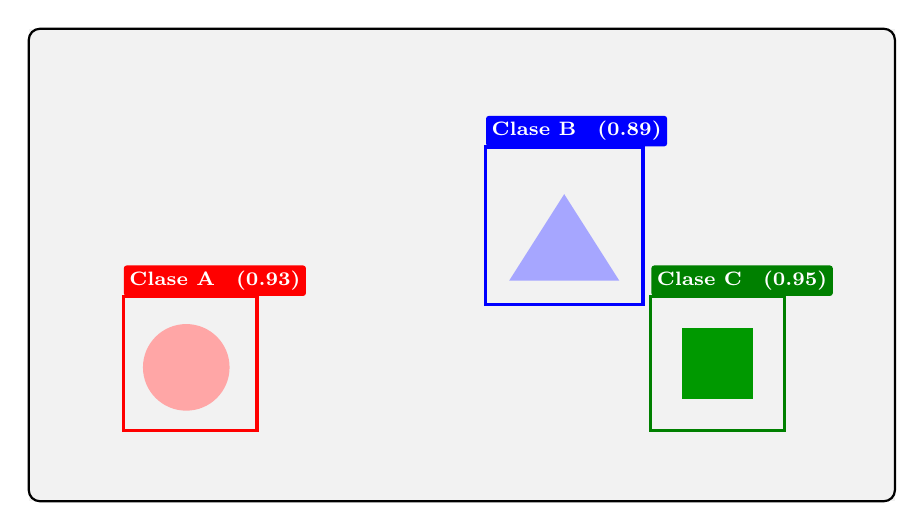
\begin{tikzpicture}[
        every node/.style={font=\small}
    ]

        % Imagen de fondo
        \fill[gray!10] (0,0) rectangle (11,6);
        \draw[rounded corners, thick] (0,0) rectangle (11,6);

        % Objetos en la escena
        % Objeto 1
        \fill[red!35] (2.0,1.7) circle (0.55);

        % Objeto 2
        \fill[blue!35] (6.8,3.9) -- (7.5,2.8) -- (6.1,2.8) -- cycle;

        % Objeto 3
        \fill[green!60!black] (8.3,1.3) rectangle (9.2,2.2);

        % Cajas delimitadoras
        \draw[red, very thick] (1.2,0.9) rectangle (2.9,2.6);
        \draw[blue, very thick] (5.8,2.5) rectangle (7.8,4.5);
        \draw[green!50!black, very thick] (7.9,0.9) rectangle (9.6,2.6);

        % Etiquetas ajustadas automáticamente al texto
        \node[
            fill=red,
            rounded corners=1pt,
            inner sep=2pt,
            anchor=south west,
            text=white,
            font=\scriptsize\bfseries
        ] at (1.2,2.6) {Clase A \, (0.93)};

        \node[
            fill=blue,
            rounded corners=1pt,
            inner sep=2pt,
            anchor=south west,
            text=white,
            font=\scriptsize\bfseries
        ] at (5.8,4.5) {Clase B \, (0.89)};

        \node[
            fill=green!50!black,
            rounded corners=1pt,
            inner sep=2pt,
            anchor=south west,
            text=white,
            font=\scriptsize\bfseries
        ] at (7.9,2.6) {Clase C \, (0.95)};

    \end{tikzpicture}
    }
    \caption{Ejemplo esquemático de detección de objetos sobre una imagen, con cajas delimitadoras, clases y niveles de confianza.}
    \label{fig:deteccion-objetos}
\end{figure}

La dificultad principal de la detección es que combina una decisión semántica y una decisión geométrica. El modelo debe reconocer la categoría de cada objeto, pero también estimar una región que represente de forma razonable su ubicación en la imagen. Esta doble exigencia hace que la tarea sea sensible a objetos pequeños, oclusiones parciales, solapamientos o elementos muy próximos entre sí. Aun así, constituye una herramienta especialmente valiosa cuando se necesita recuperar tanto la identidad de los elementos visuales como su disposición espacial dentro de la escena.


\subsection{Reconstrucción del estado observado}

Las etapas anteriores permiten obtener predicciones visuales sobre la escena capturada, pero la detección y la clasificación no constituyen por sí mismas el objetivo final del sistema. Para que la información obtenida mediante la cámara resulte útil, es necesario transformarla en una representación estructurada de lo que se observa en la partida física.

La reconstrucción del estado observado consiste en combinar la localización de los elementos visibles con la identidad asignada por los modelos de reconocimiento. En un tablero físico, la normalización geométrica permite relacionar zonas de la imagen con regiones conocidas de la superficie de juego. Sobre esta base, el proceso puede entenderse como una secuencia de transformaciones: primero se obtienen predicciones visuales sobre los elementos presentes, después se relacionan con posiciones o regiones del tablero y, finalmente, se organizan en una descripción discreta de la observación.

En el caso de \textit{Onitama}, esta transformación debe recoger principalmente dos tipos de información visual:

\begin{itemize}
    \item \textbf{Piezas}: es necesario determinar qué regiones del tablero están ocupadas e identificar el color y el tipo de cada pieza, diferenciando entre maestros y estudiantes.
    \item \textbf{Cartas}: es necesario reconocer la identidad de las cartas visibles, ya que forman parte de la información observable que condiciona el desarrollo de la partida.
\end{itemize}

El resultado de este proceso no es simplemente una imagen anotada, sino una descripción discreta de la observación visual. Sin embargo, dicha descripción debe entenderse como una estimación obtenida a partir de la imagen capturada, no como el estado lógico definitivo de la partida. La observación puede verse afectada por errores de perspectiva, oclusiones parciales, reflejos, recortes imprecisos o predicciones incorrectas de los modelos.

Por ello, la información reconstruida desde la imagen puede requerir etapas posteriores de comprobación y estabilización antes de utilizarse como entrada fiable del sistema. De este modo, la reconstrucción del estado observado actúa como enlace entre el reconocimiento visual y los módulos internos del proyecto, traduciendo las salidas de detección y clasificación en datos estructurados que puedan ser tratados computacionalmente.


%==============================================================================
% ANTECEDENTES Y TRABAJOS RELACIONADOS  (OPCIONAL)
% =============================================================================
% Para esta última seccion quizas se puede meter algo así como ejemplos de 
% proyectos similares o aplicaciones concretas de visión por computador en juegos de tablero. 
% Como el AlphaGo.
